\begin{figure}
    \centering
    \begin{figureplaceholder}
        \item[Subfig1.] This is a place holder for figure legends
    \end{figureplaceholder}
    \caption{A placeholder figure}
    \label{fig:placeholder}
\end{figure}

\begin{figure}
    \centering
    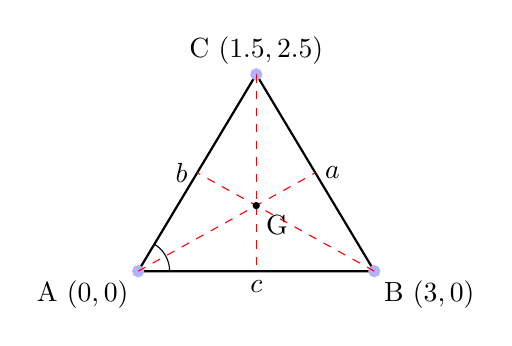
\begin{tikzpicture}
    % Example figure: labeled triangle with details

    % Draw triangle
    \draw[thick] (0,0) -- (3,0) -- (1.5,2.5) -- cycle;

    % Fill vertices
    \filldraw[blue!30!white] (0,0) circle (2pt);
    \filldraw[blue!30!white] (3,0) circle (2pt);
    \filldraw[blue!30!white] (1.5,2.5) circle (2pt);

    % Label vertices
    \node[below left] at (0,0) {A $(0,0)$};
    \node[below right] at (3,0) {B $(3,0)$};
    \node[above] at (1.5,2.5) {C $(1.5,2.5)$};

    % Name the sides
    \node[below] at (1.5,0) {$c$};
    \node[right] at (2.25,1.25) {$a$};
    \node[left] at (0.75,1.25) {$b$};

    % Draw medians
    \draw[dashed, red] (1.5,2.5) -- (1.5,0);
    \draw[dashed, red] (0,0) -- (2.25,1.25);
    \draw[dashed, red] (3,0) -- (0.75,1.25);

    % Mark centroid
    \filldraw[black] (1.5,0.833) circle (1.1pt);
    \node[below right] at (1.5,0.833) {G};

    % Show right angle at vertex A (if assumed)
    \draw (0.4,0) arc (0:60:0.4);

    \end{tikzpicture}
    \caption{A labeled triangle with details}
    \label{fig:triangle}
\end{figure}